%!TEX root = hw1.tex
\problem{4}
%Arpit in middle of problem 4. 
%Should be done in an hour. 
\paragraph{Introduction)} 
Let int  SendMessage(root,msg) be the function that transmits messages to the tree starting at the root, the function returns least number of message transmits required to transmit message to entire tree. 
for short, we call the return value of this function by SM. 
so, SM(node) = SendMessage(node,msg) = Least number of message transmits required to transmit message to the subtree starting with node. 

Consider the figure \ref{fig:4a}. Consider the node a. Children of this node are : a, b, c and d. Let us assume that we precompute the values SM(a), SM(b), SM(c) and SM(d). Intutively sending msg to node with highest SM value will overall reduce the number of message transmits needed by node a. So, Node a shoudl first send the message to node d, the node with highest SM value so far. Once the message is sent to d,  both node a and node d can together transmit the message in next cycle. But in the next cycle, the two nodes a and d will act as two different tree and that way they both will send message together.

\begin{figure}[4a]
    \centering
    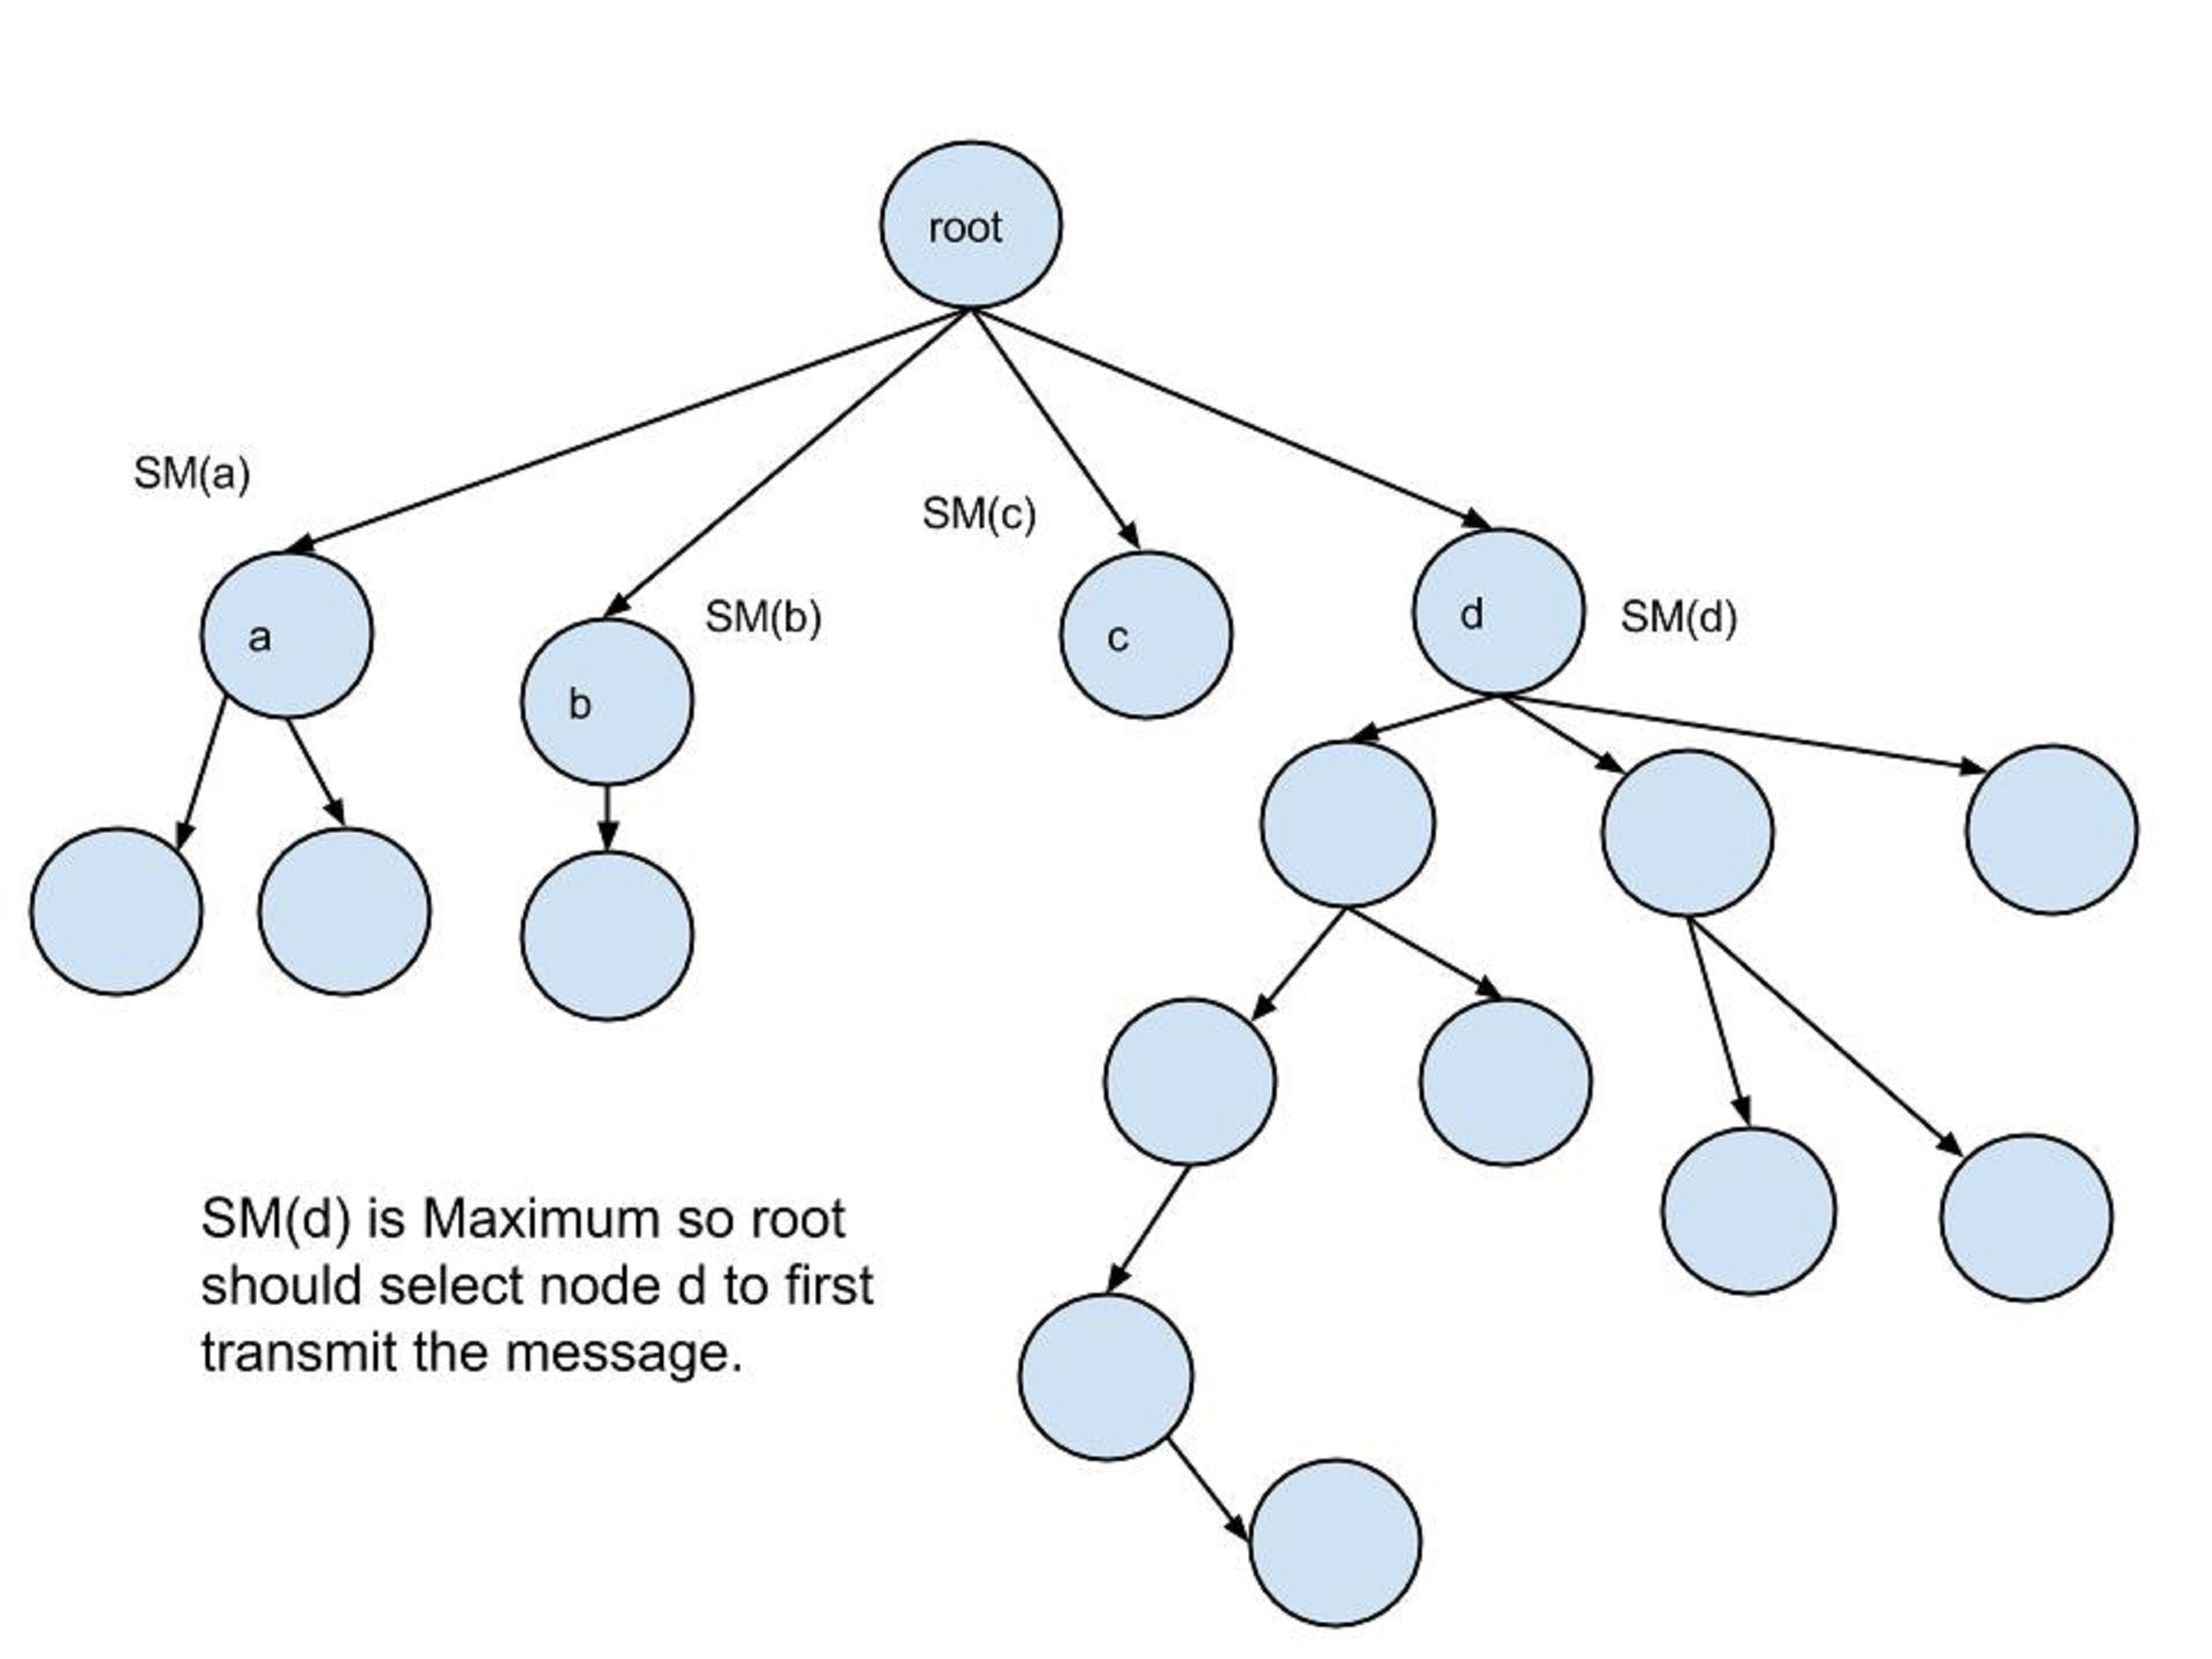
\includegraphics[scale=0.10]{4a}
    \caption{Root should first send message to node d}
    \label{fig:4a}
\end{figure}


Also, SM value depends on two factors as shown in figure \ref{fig:4b}. 

\begin{figure}[4b]
    \centering
    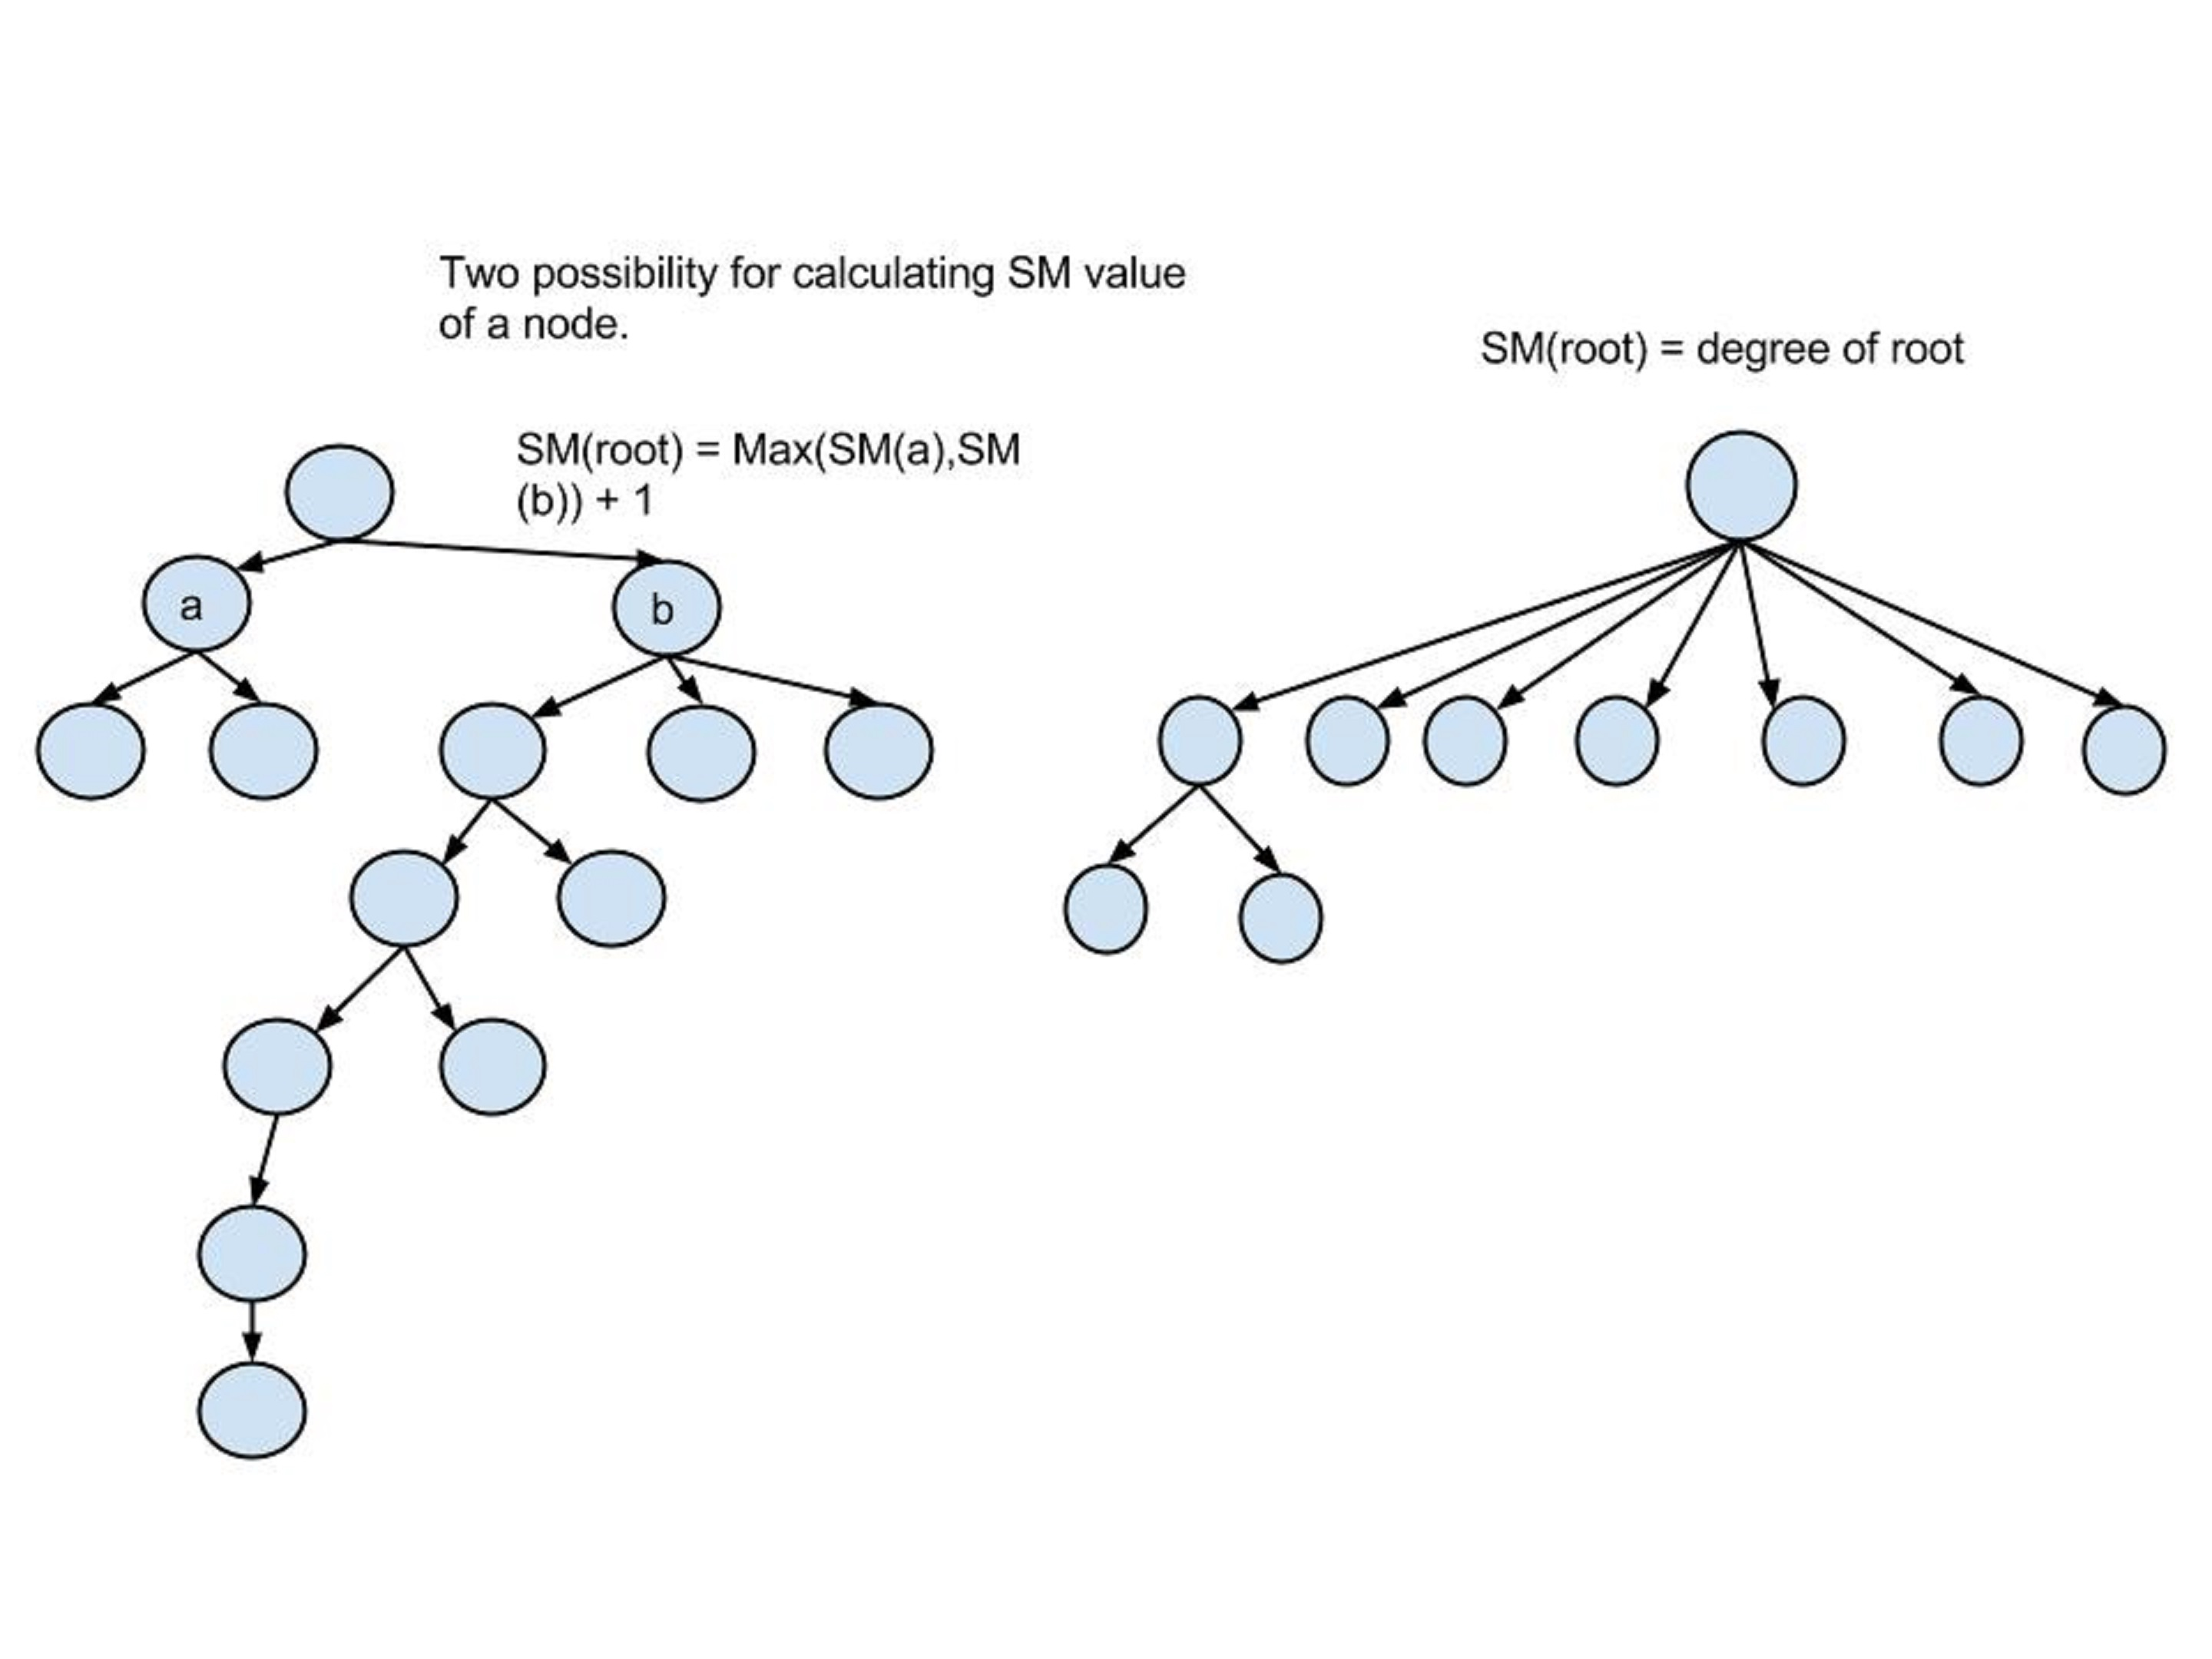
\includegraphics[scale=0.10]{4b}
    \caption{How the SM value of node can depend on two factors}
    \label{fig:4b}
\end{figure}




1) If the SM value of any child node is greate then degree of node, the maximum SM value of the child node  + 1 is the SM value of node.

2) If degree is greater then number of child nodes is the new SM Value of the node. 

The basic recursive algorith is as follows. 


\begin{algorithm}
	\caption{$Basic $ $recursive $ solution}
	\begin{algorithmic}
	  \Function{SendMessageRec}{$root$ , $msg$}
		\State $ MaxChildMsgSM = 0 $
		
		\If{$ root  == null $}
			\State $ return$ $ 0$ 	
		\EndIf
	  	\State 		
		\State $ comment: $ $ first $ $ find $ $ out $ $ maximum $ $ SMValue $  $ of $ $ all $ $ the $ $ child $ $ nodes.$		
		
		\For{$ all $ $ children $ $ of $ $ root $} 
		\State $tempMsgSM =$\Call{SendMessageRec}{$child$,$msg$}  \Comment{O(1)}
		\If {$ MaxChildMSgSM > tempMsgSM $ }		
			\State $MaxChildMSgSM = tempMsgSM$
		\EndIf
		\State	
		
		\EndFor
		
		\Return $ Max(MaxChildMsgSM + 1, $ $ Number$ $ of $ $ children $ $ of $ $ root $ $ ) $
			 
	  \EndFunction
	
	  
	\end{algorithmic}
\end{algorithm}


\paragraph{proof}
In the introduction section, we said that "Intutively sending msg to node with highest SM value will overall reduce the number of message transmits needed by the node." If we can prove this, we have proved our basic recursive algorithm as well as the dynamic programing algorithm that will follow. The SM value of a node depends on two factores. 1) If the subtrees below the node are very deep SM value is dominated by depth of the subtrees 2) The degree of the node is very high as depicted in figure and SM value of node is dominated by the number of children below the node. 

1) Assumption: \\ ASM1: Node with degree of node lower then the SM value of any of the node all the time.\\\ 

\begin{figure}[4c]
    \centering
    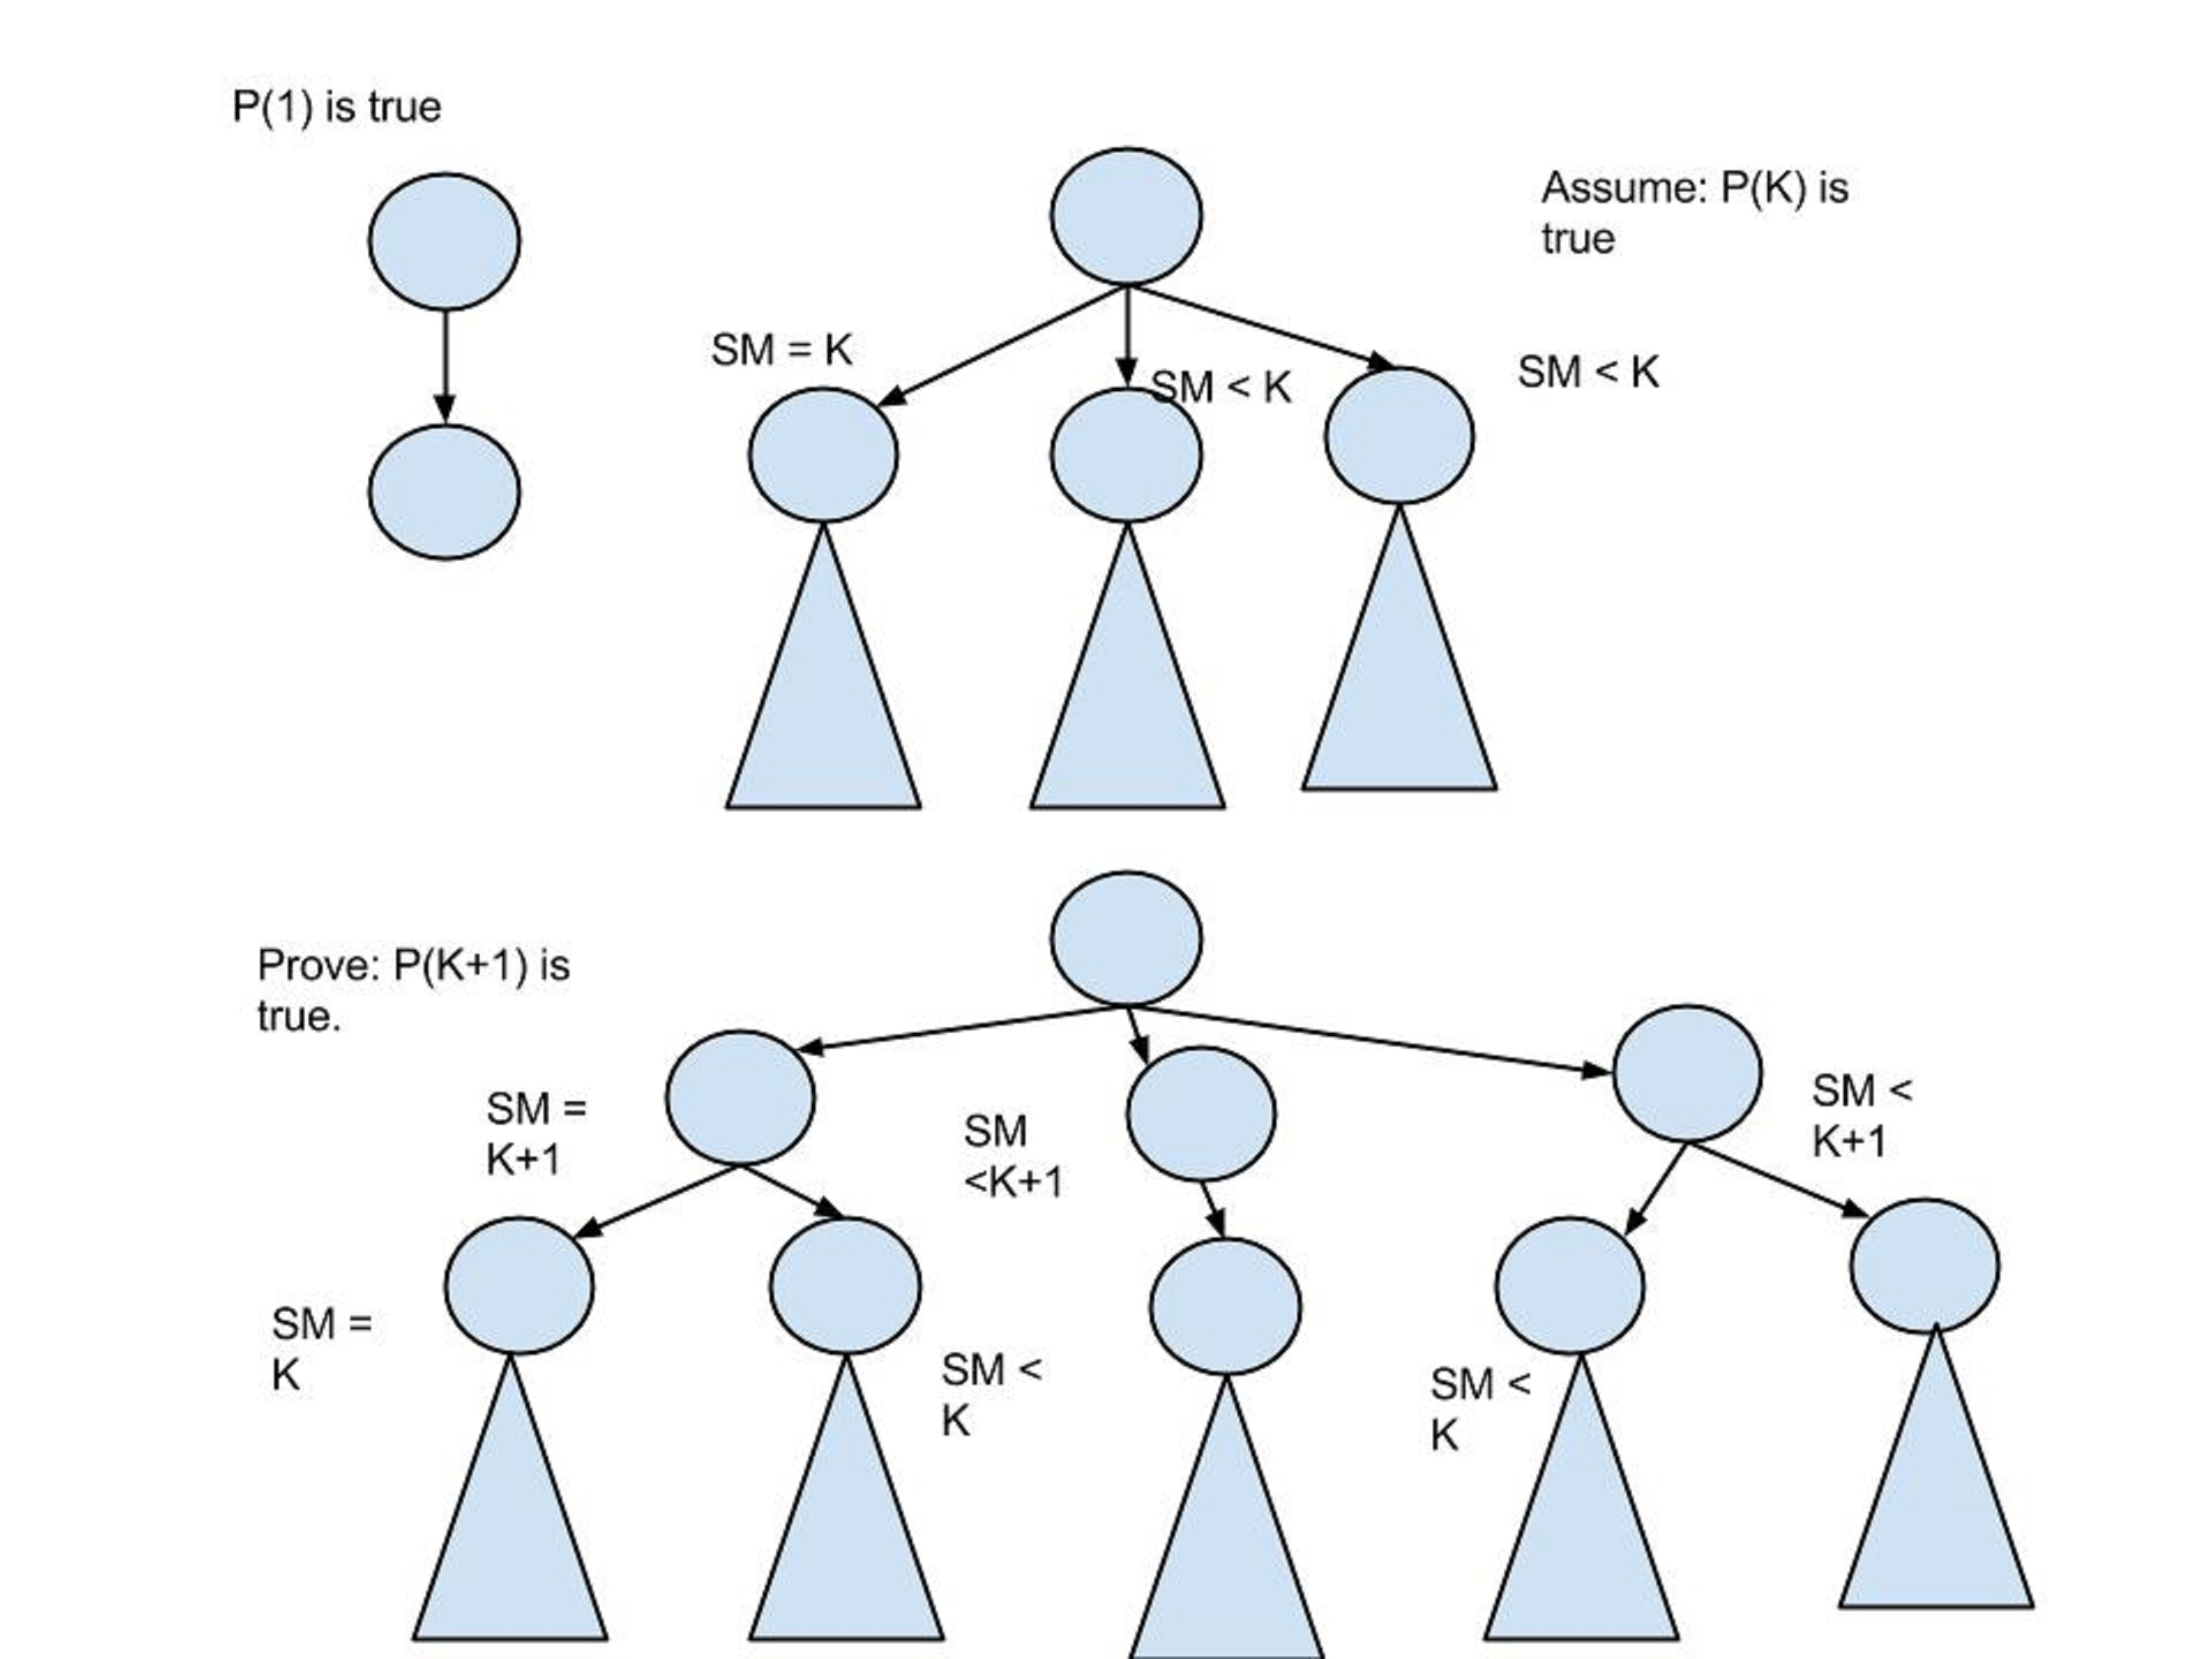
\includegraphics[scale=0.10]{4c}
    \caption{Proof with ASM 1}
    \label{fig:4c}
\end{figure}

Taking induction on highest SM value of children of node. 
P(K) : For any node, If the highest SM value of one of its children is K, sending message to that child minimizes the total message tranmits needed for that node.\\ 

Proof scenario for ASM1 is depicted in Figure \ref{fig:4c}

P(1) is true. Under the assumption ASM1, the only possible tree is as shown in figure.
For this tree, P(1) is true as total number of messages transmits needed is 1. 

Assume P(K) is true.  As shown in figure, for all child nodes of node, tranmitting message to the node with highest SM value K, the total message transmits are minimum.\\

Prove that P(K+1) is true. As shown in figure 3 below, the one of the node has highest SM value of K + 1 while other nodes has SM value of <K + 1. \\

Under assumption ASM1, for the subtree of node with SM value K +1, there exists a node with SM value of K. while for other nodes as b, c etc. all such noes has SM values of < K. Also P(K) is true, so total number of message transmits minimizes when message is first transmitted to node with SM value of K then nodes with SM value of < K. The message transmits at a, b, c ... require one more message tranmits than the highest SM value of their subtrees and that maximizes for node a, with SM value of K + 1. So, P(K + 1) is true. \\

2) Assumption ASM2: Node with degree of node higher then SM value of any node all the time. 
Taking induction on degree of node. The situation is depicted in figure \ref{fig:4d}. 

\begin{figure}[4d]
    \centering
    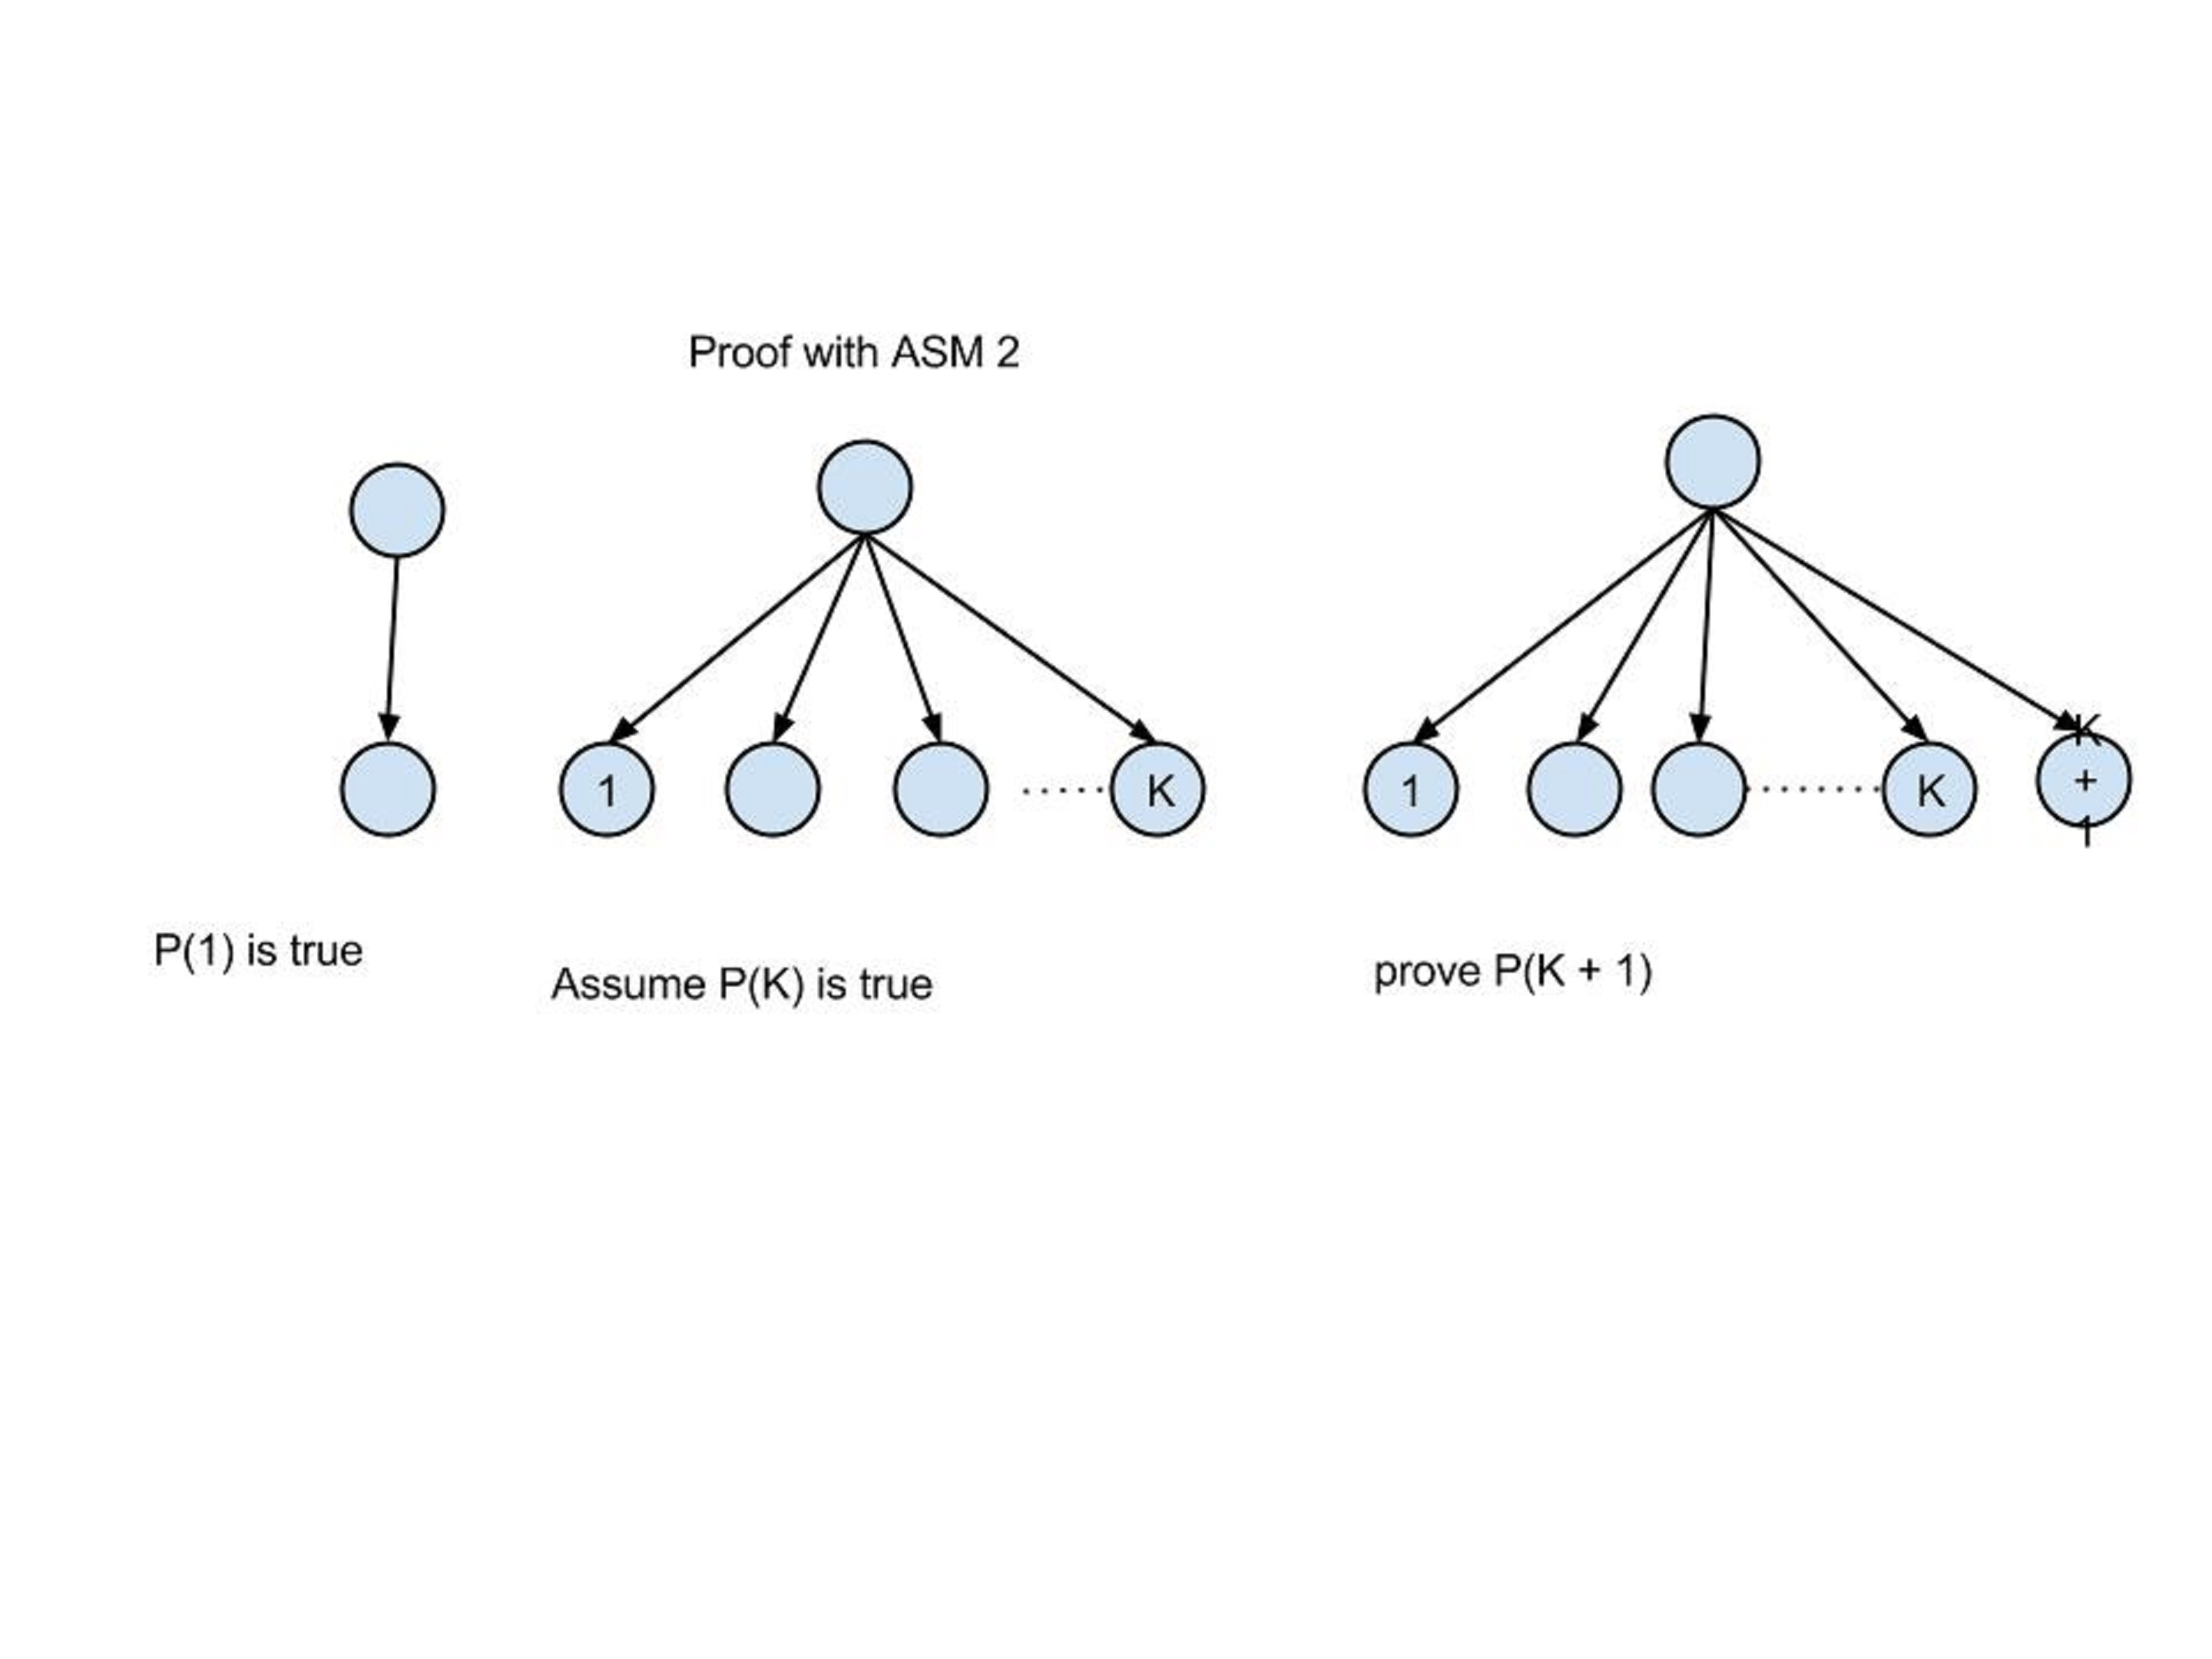
\includegraphics[scale=0.10]{4d}
    \caption{Proof with ASM2}
    \label{fig:4d}
\end{figure}
 
P(K): For any node, the highest degree of  its children is K, SM value of that node is K. 

P(1) is trivialy true. 
Assume P(K) is true. If the degree of node is k, and it is more then any of the SM value, then SM value of that node is K.  

Prove P(K + 1) is true. 
Adding one node to the child node, will require to transmit one more message, and ASM2 is still true that means that we will need to transmit K + 1 messages and hence P(K + 1) is true and SM value of node is degree of node.  

3) Most generic case, dropping both the assumptioin. 
Any node will follow in case 1 and case 2. The only issue now is the possibility of node's SM value changing based on degree of node or SM value of its subtree. (Before it was strictly one of the case). Using the same arguments as used in case 1 and case 2, and using maximum values between {degree of nodes, Highest SM  value of subtree} and handling ties by randomly choosing any of the method, our proof stil holds. 

\paragraph{Dynamic programming algorithm}
For dynamic programming algorithm, we will change the tree node as following \\
TreeNode(\\
List of childNodes,  \\
int SMValue, \\
bool visited \\
)

bool visited is used to prevent from visiting any node again. (Basically we are creating seperate trees)
int SMValue holds the computed SMValue for the node. 

Initialize() \\
method initializes following values of all the nodes. \\
SMValue = -1; \\
visited = false;\\


Though it may require O(n) time to initialize, Under the assumption that the above two operations are quite cheap compared to SendMessage operation, we can consider the cost of initialize() method to be constant. Even if we consider the cost O(n), this will not change the overall complexity of complete algortihm. \\

After initilization, SendMessage(root,msg) method will be called. 




\begin{algorithm}
	\caption{$Dynamic $ $programming$ solution}
	\begin{algorithmic}
	  \Function{SendMessage}{$root$ , $msg$}
		\State $ MaxChildMsgSM = 0 $
		\State $ ChildWithMaxMsgDepth = null $
		\If{$ root  == null $}
			\State $ return$ $ 0$ 	
		\EndIf
	  	\State 		
		\State $comment: $ $ first $ $ find $ $ out $ $ maximum $ $ SMValue $  $ of $ $ all $ $ the $ $ child $ $ nodes.$		
		
		\For{$ all $ $ children $ $ of $ $ root $}
		
		\State 
		\If{$ child.visited == true $}
			\State do nothing
		\Else
		\State		
		
		\If{$ child.SMValue !=  -1$}
			 \State			 
			 \If{ $ child.SMValue > MaxChildMsgSM $ }
			 	\State $ MaxChildMsgSM = child.SMValue$
				\State $ ChildWithMaxMsgDepth = child $
			  \EndIf
				\State
	     \EndIf
	     \If{$ child.SMValue == -1 $}
		     	
	     	\State $tempSMValue =  $\Call{SendMessage}{$child$,$msg$} \Comment{O(1)}
	     	\State $child.SMValue = tempSMValue$
	     	\If{ $ child.SMValue > MaxChildMsgSM $ }
			 	\State $ MaxChildMsgSM = child.SMValue$
				\State $ ChildWithMaxMsgDepth = child $
				\State $ child.visited = true $
			\EndIf
		\EndIf		
		\EndIf
			
		\EndFor
		
		
		
		\Return $ Max(MaxChildMsgSM + 1,$ $ Number$ $ of $ $ children $ $ of $ $ root $ $ ) $
			 				
		
		
	  \EndFunction
	
	  
	\end{algorithmic}
\end{algorithm}

\paragraph{Runtime analysis}

Our assumption in this analysis is that cost of sending message to a node is much higher then any other cost. Under this assumption, as shown in algorithm, every node is sent message only once. Once it is sent message, it is marked as visited and essentially we are detaching that node from its parent node for further manipulation. so every node will recieve message once from its parent. so time complexity of this algoritm is O(n). 

We have added two new data to each node. Added SMValue field to preserve the SMValue calculated for each node. Added visited boolean value to detach a node from its parent node from further consideration, once it is already sent a message. so we have added 2 extra fields for each node. So, space complexity of this algorithm is 2n and hence O(n).  

In case findning number of children nodes is costly operation also, then we can compute it within algorithm by adding a new field, NumberofChildren to each node of tree and in that case, algorithm's space complexity will be in terms of 3n but it will still reamin O(n)


